\chapter{正则化与模型选择}\label{chapter:9}

\section{正则化}\label{sec:9.1}

回顾第 \ref{sec:8.1} 节中讨论的,过拟合通常是由于使用了过于复杂的模型导致的,我们需要选择适当的模型复杂度以达到最优的偏差-方差权衡。当模型复杂度用参数数量衡量时,我们可以改变模型的规模(例如,神经网络的宽度)。然而,衡量模型复杂度的正确且有信息量的方式可以是参数的函数(例如,参数的 $\ell_2$ 范数),这可能不一定取决于参数的数量。在这种情况下,我们将使用正则化,这是一种重要的机器学习技术,用于控制模型复杂度并防止过拟合。

正则化通常涉及在训练损失/代价函数中添加一个附加项,称为正则项,这里用 $R(\theta)$ 表示:
\begin{equation}
    J_\lambda(\theta) = J(\theta) + \lambda R(\theta)
    \label{eq:9.1}
\end{equation}
这里,$J_\lambda$ 通常被称为正则化损失,$\lambda \geq 0$ 被称为正则化参数。正则项 $R(\theta)$ (在几乎所有情况下)是一个非负函数。在经典方法中,$R(\theta)$ 纯粹是参数 $\theta$ 的函数,但一些现代方法允许 $R(\theta)$ 依赖于训练数据集。\footnote{为了简洁起见,这里的记号省略了对训练数据集的依赖性——$J(\theta)$ 显然需要依赖于训练数据集。}

正则项 $R(\theta)$ 通常被选择为衡量模型 $\theta$ 复杂度的某种度量。因此,在使用正则化损失时,我们的目标是找到一个既能很好地拟合数据(即具有小的损失 $J(\theta)$)又具有小的模型复杂度(即小的 $R(\theta)$)的模型。这两个目标之间的平衡由正则化参数 $\lambda$ 控制。当 $\lambda = 0$ 时,正则化损失等同于原始损失。当 $\lambda$ 是一个足够小的正数时,最小化正则化损失也可以有效地最小化原始损失,同时利用正则项来区分那些原始损失相同的解。当正则项非常大时,原始损失不再有效(并且模型很可能具有很大的偏差)。

最常用的正则化可能是 $\ell_2$ 正则化,其中 $R(\theta) = \frac{1}{2}\|\theta\|_2^2$。它鼓励优化器找到一个 $\ell_2$ 范数较小的模型。在深度学习中,这通常被称为\textbf{权重衰减 (weight decay)},因为在正则化损失上进行学习率为 $\eta$ 的梯度下降,等价于将 $\theta$ 乘以一个标量因子 $1 - \eta\lambda$ 收缩/衰减后,使用标准梯度:
\begin{align}
    \theta &\leftarrow \theta - \eta \nabla J_\lambda(\theta) = \theta - \eta \lambda \theta - \eta \nabla J(\theta) \nonumber \\
    &= \underbrace{(1 - \eta \lambda)\theta}_{\text{权重衰减}} - \eta \nabla J(\theta)
    \label{eq:9.2}
\end{align}

除了鼓励更简单的模型之外,正则化还可以对模型参数施加归纳偏置或结构。例如,假设我们先验地认为真实模型参数中非零项的数量很少\footnote{对于线性模型,这意味着模型只使用输入的少数几个坐标来做出准确的预测。}——这通常被称为模型的稀疏性——就可以对 $\theta$ 的非零项数量施加正则化,记作 $\|\theta\|_0$,从而利用这种先验。施加额外的参数结构会缩小我们的搜索空间,并使模型族的复杂度变小——例如,稀疏模型族可以被认为比所有模型族具有更低的复杂度——因此往往会带来更好的泛化能力。另一方面,强烈施加额外的结构可能会增加偏差的风险。例如,如果强烈地对稀疏性进行正则化,但是稀疏模型不能准确地预测,我们将会遭受很大的偏差(类似于第 \ref{sec:8.1} 节中使用线性模型去学习由二次函数表示的数据的情况)。

参数的稀疏性不是参数的连续函数,因此无法通过(随机)梯度下降对其进行优化。一个常见的松弛方法是使用 $R(\theta) = \|\theta\|_1$ 作为替代。\footnote{存在丰富的理论工作解释了为什么 $\|\theta\|_1$ 是稀疏性的良好替代,但这超出了本课程的范围。直观地说:假设参数在单位球面上,具有最小 $\ell_1$ 范数的参数也碰巧是只有 1 个非零坐标的最稀疏参数。因此,在某种程度上,稀疏性和 $\ell_1$ 范数给出了相同的极值点。}

对于线性模型,$R(\theta) = \|\theta\|_1$(也称为 LASSO)和 $R(\theta) = \frac{1}{2}\|\theta\|_2^2$ 可能是最常用的正则化项。其他范数和范数的幂有时也会被使用。$\ell_2$ 范数正则化在核方法中更为常用,因为 $\ell_1$ 正则化通常与核技巧不兼容(最优解不能写成特征内积的函数)。

在深度学习中,最常用的正则化项是 $\ell_2$ 正则化或权重衰减。其他常见的正则化方法包括 dropout、数据增强、对权重矩阵的谱范数进行正则化以及对模型的 Lipschitz 性进行正则化等。深度学习中的正则化是一个活跃的研究领域,并且我们还知道还有一个隐式的正则化来源,这将在下一节中讨论。

\section{隐式正则化效应 (选读)}\label{sec:9.2}

优化器的隐式正则化效应,或者说隐式偏置或算法正则化,是在深度学习时代观察到的一个新概念/现象。它主要指的是优化器可以在正则化损失所施加的结构之外,隐式地对参数施加结构。

在大多数经典设置中,损失或正则化损失具有唯一的全局最小值,因此任何合理的优化器都应该收敛到该全局最小值,并且不施加任何额外的偏好。然而,在深度学习中,通常损失或正则化损失具有多个(近似)全局最小值,不同的优化器可能收敛到不同的全局最小值。尽管这些全局最小值具有相同或相似的训练损失,但它们的性质可能不同,并且泛化性能也可能显著不同。参见图 9.1 和 9.2 及其说明文字,以了解插图和一些实验结果。例如,某个全局最小值可能比其他全局最小值产生更具 Lipschitz 性或更稀疏的模型,从而具有更好的测试误差。结果表明,许多常用的优化器(或其组成部分)倾向于或偏向于寻找具有某些特性的全局最小值,从而带来更好的测试性能。

\begin{figure}[H]
    \centering
    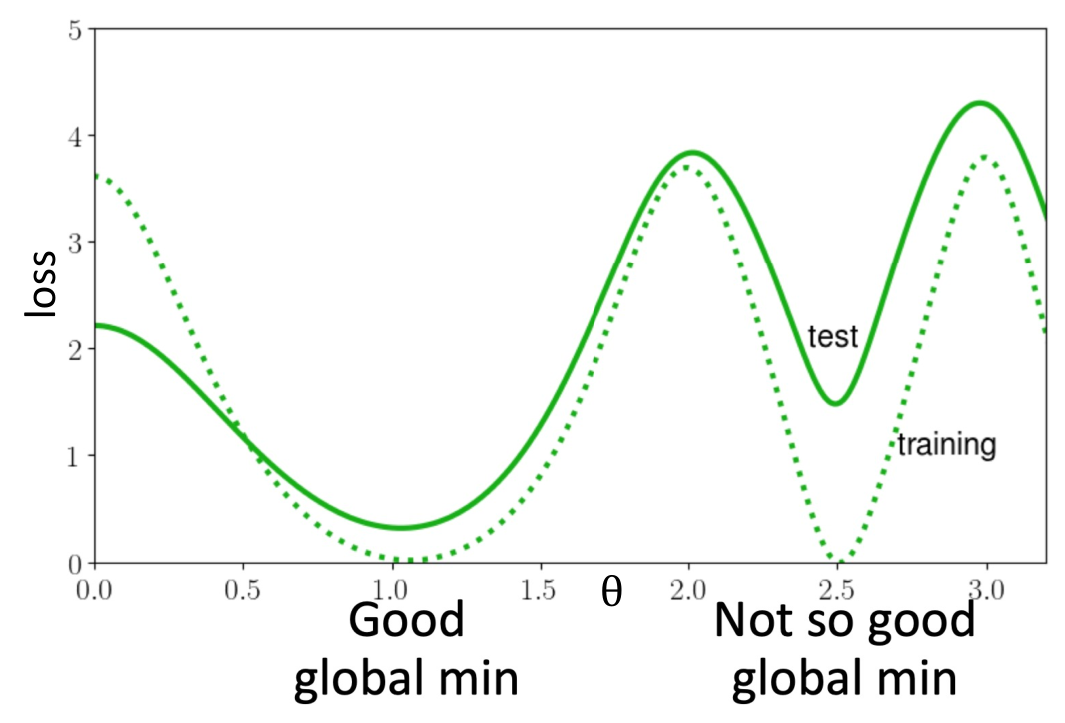
\includegraphics[width=0.6\textwidth]{figs/global_minima.png}
    \caption{在训练损失上的全局最小点的测试性能不相同的图示。}
    \label{fig:9.1}
\end{figure}

\begin{figure}[H]
    \centering
    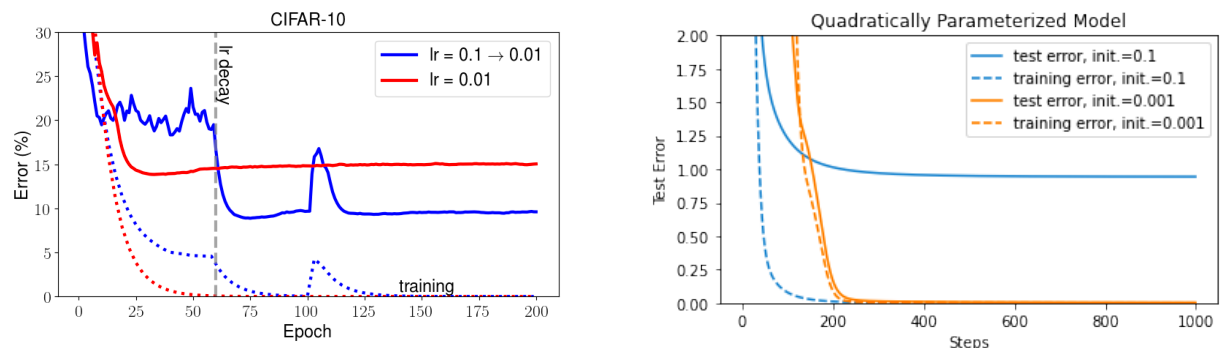
\includegraphics[width=0.9\textwidth]{figs/global_minima_nn.png}
    \caption{\textbf{左:}在 CIFAR-10 数据集上,使用两种不同学习率调度方案训练的神经网络的性能。尽管两个实验使用了完全相同的正则化损失,并且优化器完美地拟合了训练数据,但模型的泛化性能差异很大。\textbf{右}:在另一个合成数据集上,使用不同初始化的优化器具有相同的训练误差,但泛化性能不同。\protect\footnotemark}
\end{figure}
\footnotetext[4]{设置与 \cite{woodworth2020kernel} 和 \cite{haochen2020shape} 一致。}

总而言之,所要传达的关键信息是,优化器的选择不仅影响训练损失的最小化,还施加了隐式正则化并影响模型的泛化能力。即使当前的优化器已经完美地收敛到较小的训练误差,也可能仍然需要调整优化器以获得更好的泛化性能。

人们可能会想知道优化器的哪些组成部分偏向于哪种类型的全局最小值,以及哪种类型的全局最小值可能具有更好的泛化能力。这些是研究人员正在积极探索的开放性问题。经验和理论研究已经提供了一些线索和启发式方法。在许多(但不是全部)情况下,在那些优化能够成功最小化训练损失的设置中,使用较大的初始学习率、较小的初始化、较小的批量大小和动量似乎有助于偏向于更具泛化能力的解。一个猜想(在某些简化情况下可以证明)是,优化过程中的随机性有助于优化器找到更平坦的全局最小值(损失曲率较小的全局最小值),而平坦的全局最小值往往会产生更具 Lipschitz 性和更好泛化能力的模型。形式化地刻画隐式正则化效应仍然是一个具有挑战性的开放性研究问题。

\section{通过交叉验证选择模型}\label{sec:9.3}

假设我们正在为一个学习问题选择几种不同的模型。例如,我们可能正在使用多项式回归模型 $h_\theta(x) = g(\theta_0 + \theta_1 x + \theta_2 x^2 + \dots + \theta_k x^k)$,并希望决定 $k$ 应该取 0, 1, ..., 或 10 中的哪个值。我们如何自动选择一个模型,使其在偏差和方差这对孪生罪恶之间取得良好权衡?\footnote{考虑到我们在之前的笔记中说过偏差和方差是截然不同的两种“野兽”,有些读者可能会想知道我们在这里是否应该称它们为“孪生”罪恶。也许最好将它们视为非同卵双胞胎。不过“偏差和方差这对异卵孪生罪恶”这个短语听起来不太顺口。} 另外,假设我们想自动选择局部加权回归的带宽参数 $\tau$,或者 $\ell_1$ 正则化 SVM 的参数 $C$,该如何做?

为了具体起见,在这些笔记中,我们假设我们有一些有限的模型集合 $\mathcal{M} = \{M_1, \dots, M_d\}$,我们正尝试从中进行选择。例如,在上面的第一个例子中,模型 $M_i$ 将是一个 $i$ 次多项式回归模型。(推广到无限 $\mathcal{M}$ 并不难。\footnote{如果我们正在从无限的模型集合中进行选择,例如对应于带宽 $\tau \in \mathbb{R}^+$ 的所有可能值,我们可以对 $\tau$ 进行离散化,只考虑其有限个可能值。更普遍地,这里描述的大多数算法都可以看作是在模型空间中执行优化搜索,而且我们也可以在无限模型类别上执行这种搜索。})另外,如果我们正在决定是使用 SVM、神经网络还是逻辑回归,那么 $\mathcal{M}$ 可能包含这些模型。

\subsection*{交叉验证}

假设我们像往常一样,给定一个训练集 $S$。考虑到我们对经验风险最小化的了解,以下是基于经验风险最小化进行模型选择的一种初步算法:

\begin{enumerate}
    \item 在 $S$ 上训练每个模型 $M_i$,得到假设 $h_i$。
    \item 选择训练误差最小的假设。
\end{enumerate}

这个算法\textit{不 (not)} 起作用。考虑选择多项式的幂次。多项式的幂次越高,它就越能更好地拟合训练集 $S$,从而训练误差越低。因此,这种方法总是会选择高方差、高幂次的多项式模型,正如之前所述,这通常是一个糟糕的选择。

这里有一个效果更好的算法:叫做\textbf{留出交叉验证 (hold-out cross validation)}(也称为\textbf{简单交叉验证 (simple cross validation)})中,算法执行以下步骤:

\begin{enumerate}
    \item 随机将 $S$ 分割成 $S_{\text{train}}$(例如,70\% 的数据)和 $S_{\text{cv}}$(剩余的 30\%)。这里的 $S_{\text{cv}}$ 称为留出交叉验证集。
    \item 仅在 $S_{\text{train}}$ 上训练每个模型 $M_i$,得到一些假设 $h_i$。
    \item 选择并输出在留出交叉验证集上误差 $\hat{\varepsilon}_{S_{\text{cv}}}(h_i)$ 最小的假设 $h_i$。(这里 $\hat{\varepsilon}_{S_{\text{cv}}}(h)$ 表示假设 $h$ 在 $S_{\text{cv}}$ 中的例子上的平均误差。)留出集上的误差也称为验证误差。
\end{enumerate}

通过在模型未训练过的例子集合 $S_{\text{cv}}$ 上进行测试/验证,我们获得了每个假设 $h_i$ 的真实泛化/测试误差的更好估计。因此,这种方法本质上是选择具有最小估计泛化/测试误差的模型。验证集的大小取决于可用例子的总数。通常,留出交叉验证中使用的验证集数据量占总数据量的 1/4 到 1/3,其中 30\% 是一个典型的选择。然而,当总数据集非常大时,只要验证例子的绝对数量足够多,验证集可以占总例子的一小部分。例如,ImageNet 数据集有大约 1M 训练图像,验证集有时设置为 50K 图像,仅占总例子的约 5\%。

可选地,算法中的步骤 3 也可以替换为根据 $\arg \min_i \hat{\varepsilon}_{S_{\text{cv}}}(h_i)$ 选择模型 $M_i$,然后使用整个训练集 $S$ 重新训练 $M_i$。(这通常是一个好主意,除了一个例外,即对初始条件和/或数据的扰动很敏感的学习算法。对于这些方法,模型 $M_i$ 在 $S_{\text{train}}$ 上表现良好并不一定意味着它在 $S_{\text{cv}}$ 上也会表现良好,并且最好放弃重新训练这一步。)

使用留出交叉验证的缺点是它“浪费”了大约 30\% 的数据。就算我们选择在整个训练集上重新训练,但如果我们试图寻找一个性能良好的模型,却只有 $0.7n$ 个训练样本而不是完整的 $n$ 个训练样本,那么这种“浪费”依然存在。虽然在数据丰富廉价的情况下这很好,但在数据稀缺的情况下(比如 $n=20$ 时),我们希望采取更有效的方法。

这里有一种称为 \textbf{$k$ 折交叉验证 ($k$-fold cross validation)} 的方法,它每次保留更少的数据:

\begin{enumerate}
    \item 随机将 $S$ 分割成 $k$ 个不相交的子集,每个子集包含 $m/k$ 个训练样本。我们将这些子集称为 $S_1, \dots, S_k$。
    \item 对于每个模型 $M_i$,我们按如下方式评估它:
    \begin{itemize}
        \item[] 对于 $j=1, \dots, k$
        \begin{itemize}
            \item[] 在 $S_1 \cup \dots \cup S_{j-1} \cup S_{j+1} \cup \dots \cup S_k$ 上训练模型 $M_i$(即,在除 $S_j$ 外的所有数据上训练),得到一些假设 $h_{ij}$。
            \item[] 在 $S_j$ 上测试假设 $h_{ij}$,得到 $\hat{\varepsilon}_{S_j}(h_{ij})$。
        \end{itemize}
        \item[] 然后,模型 $M_i$ 的估计泛化误差计算为 $\hat{\varepsilon}_{S_j}(h_{ij})$ 的平均值(对 $j$ 取平均)。
    \end{itemize}
    \item 选择估计泛化误差最低的模型 $M_i$,并在整个训练集 $S$ 上重新训练该模型。得到的假设作为最终输出。
\end{enumerate}

这里通常选择的折数是 $k=10$。每次保留的数据比例现在是 $1/k$,比之前小得多——这个过程也可能比留出交叉验证的计算成本更高,因为现在需要对每个模型训练 $k$ 次。

虽然 $k=10$ 是一个常用的选择,但在数据非常稀缺的问题中,有时我们会使用极端的选择 $k=m$,以便每次保留尽可能少的数据。在这种设置下,我们会在 $S$ 中除了一个训练例子之外的所有例子上重复训练,并在那个保留的例子上进行测试。然后将得到的 $m=k$ 个误差平均起来,以获得模型泛化误差的估计。这种方法也有自己的名字,由于我们每次只保留一个训练样本,这种方法称为\textbf{留一交叉验证 (leave-one-out cross validation)}。

最后,虽然我们把这些交叉验证当作选择模型的方法,它们也可以用于评估\textit{单个 (single)} 模型或算法。例如,如果您实现了一些学习算法并想估计它在您的应用程序中的表现如何(或者如果您发明了一种新的学习算法并想在技术论文中报告它在各种测试集上的表现),交叉验证是一种合理的方法。

\section{贝叶斯统计与正则化}\label{sec:9.4}

本节我们将讨论对抗过拟合的另一个工具。

之前我们讨论了使用最大似然估计(MLE)进行参数拟合,并根据以下公式选择参数:
\[
    \theta_{\text{MLE}} = \arg \max_\theta \prod_{i=1}^n p(y^{(i)} | x^{(i)}; \theta).
\]

在随后的讨论中,我们将 $\theta$ 视为一个未知参数。这种将 $\theta$ 视为\textit{常数但未知 (constant-valued but unknown)} 的观点在\textbf{频率派 (frequentist)} 统计学中被采用。在频率派观点中,$\theta$ 不是随机的——它只是未知的——而我们的任务是利用统计程序(例如最大似然)来估计这个参数。

解决参数估计问题的另一种方法是采用\textbf{贝叶斯 (Bayesian)} 的世界观,并将 $\theta$ 视为一个\textit{随机变量 (random
variable)},其值是未知的。在这种方法中,我们会指定一个\textbf{先验分布 (prior distribution)} $p(\theta)$,它表达了我们对参数的“先验观念”。给定一个训练集 $S = \{(x^{(i)}, y^{(i)})\}_{i=1}^n$,当被要求对一个新的 $x$ 值进行预测时,我们可以计算参数的后验分布
\begin{align}
    p(\theta | S) &= \frac{p(S | \theta) p(\theta)}{p(S)} \notag \\
    &= \frac{(\prod_{i=1}^n p(y^{(i)} | x^{(i)}, \theta)) p(\theta)}{\int_\theta (\prod_{i=1}^n p(y^{(i)} | x^{(i)}, \theta)) p(\theta) d\theta} \label{eq:9.3}
\end{align}
在上述公式 \eqref{eq:9.3} 中,$p(y^{(i)} | x^{(i)}, \theta)$ 可以来自所研究的学习问题所采用的任何模型。例如,如果使用贝叶斯逻辑回归,那么可能会选择 $p(y^{(i)}|x^{(i)}, \theta) = h_\theta(x^{(i)})^{y^{(i)}} (1-h_\theta(x^{(i)}))^{1-y^{(i)}}$,其中 $h_\theta(x^{(i)}) = 1/(1 + \exp(-\theta^T x^{(i)}))$。\footnote{因为现在 $\theta$ 被视为一个随机变量,所以将它作为条件是可以的,写作 $p(y|x, \theta)$ 而不是 $p(y|x; \theta)$。}

当给定一个新的测试样本 $x$ 并要求对其进行预测时,可以使用关于 $\theta$ 的后验分布计算类别标签上的后验分布:
\begin{equation}
    p(y|x, S) = \int_\theta p(y|x, \theta) p(\theta|S) d\theta
    \label{eq:9.4}
\end{equation}
在上述公式 \eqref{eq:9.4} 中,$p(\theta|S)$ 来自公式 \eqref{eq:9.3}。因此,例如,如果目标是预测给定 $x$ 时 $y$ 的期望值,那么有\footnote{如果 $y$ 是离散值,下面的积分将被求和代替。}
\[    
    E[y|x, S] = \int_y y p(y|x, S) dy
\]

所概述的这个过程可以被认为是进行“完全贝叶斯”预测,其中模型的预测是通过对 $\theta$ 的后验分布 $p(\theta|S)$ 求平均来计算的。不幸的是,通常情况下计算这个后验分布的计算成本非常高。这是因为这需要对公式 \eqref{eq:9.3} 中的(通常是高维的)$\theta$ 进行积分,而这通常无法得到闭式解。

因此,实践中将转而近似 $\theta$ 的后验分布。一种常见的近似方法是用一个单点估计来代替 $\theta$ 的后验分布(如公式 \eqref{eq:9.4} 中所示)。$\theta$ 的\textbf{最大后验 (maximum a posteriori, MAP)} 估计由下式给出:
\begin{equation}
    \theta_{\text{MAP}} = \arg \max_\theta \prod_{i=1}^n p(y^{(i)} | x^{(i)}, \theta) p(\theta).
    \label{eq:9.5}
\end{equation}
注意,这与 $\theta$ 的最大似然估计(MLE)的公式相同,只是在末尾多了一个先验项 $p(\theta)$。

在实际应用中,先验 $p(\theta)$ 的一个常见选择是假设 $\theta \sim \mathcal{N}(0, \tau^2 I)$。使用这种先验选择,拟合的参数 $\theta_{\text{MAP}}$ 的范数将小于通过最大似然选择的范数。在实践中,这使得贝叶斯 MAP 估计对过拟合不那么敏感,优于参数的最大似然估计。例如,贝叶斯逻辑回归被证明是文本分类的有效算法,即使在文本分类中通常有 $d \gg n$。